\documentclass{article}
\usepackage{graphicx,psfrag,epsfig,epsf,latexsym,hhline,amsmath,amssymb,multirow}
\usepackage[usenames,dvipsnames]{pstricks}
\usepackage{pst-plot}
\usepackage{pstricks-add}
\usepackage{color}
\usepackage{stmaryrd}
\usepackage{makecell}

\interdisplaylinepenalty=2500
\usepackage{graphicx}
\usepackage{amsthm}
\usepackage{footnote}

\usepackage{blindtext}
\usepackage{etoolbox}

\usepackage{tikz}
\usepackage{pgfplots}
\usepgflibrary{shapes}
\usetikzlibrary{arrows,shapes,chains,matrix,positioning,scopes,patterns	}
\pgfplotsset{compat=newest}
\pgfplotsset{plot coordinates/math parser=false}

\begin{document}
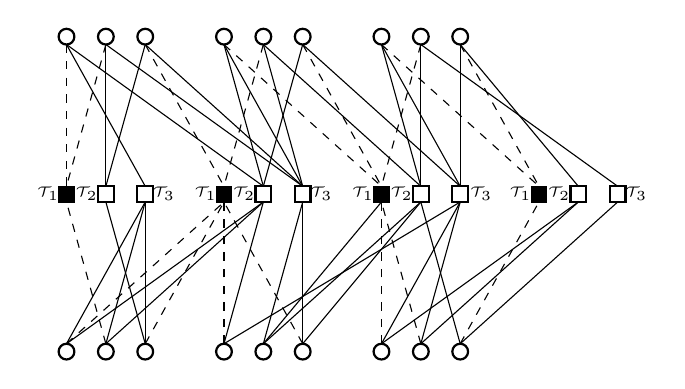
\begin{tikzpicture}
\draw [fill=black] (0.1,0.1) rectangle (-0.1,-0.1); 
\node [left,font=\tiny] at (0.03,0){$\mathcal{T}_{1}$} ;

	\draw[thick,black] (0,2) circle (0.1);  \draw[thick,black] (0,-2) circle (0.1);
	\draw[thick,black] (0.6,0.1) rectangle (0.4,-0.1);\node [left,font=\tiny] at (0.52,0){$\mathcal{T}_{2}$} ;
  	\draw[thick,black] (0.5,2) circle (0.1);  \draw[thick,black] (0.5,-2) circle (0.1);
	\draw[thick,black] (1.1,0.1) rectangle (0.9,-0.1); \node [right,font=\tiny] at (0.97,0){$\mathcal{T}_{3}$} ;
 	\draw[thick,black] (1,2) circle (0.1);  \draw[thick,black] (1,-2) circle (0.1);

\draw [dashed] (0,1.9) -- (0,0.1);  \draw (0,1.9) -- (2.5,0.1); \draw (0,1.9) -- (1,0.1);
\draw [dashed] (0.5,1.9) -- (0,0.1);  \draw (0.5,1.9) -- (0.5,0.1); \draw (0.5,1.9) -- (3,0.1);
\draw [dashed] (1,1.9) -- (2,0.1);  \draw (1,1.9) -- (0.5,0.1); \draw (1,1.9) -- (3,0.1);

\draw [dashed] (0,-1.9) -- (2,-0.1);  \draw (0,-1.9) -- (2.5,-0.1); \draw (0,-1.9) -- (1,-0.1);
\draw  [dashed] (0.5,-1.9) -- (0,-0.1);  \draw (0.5,-1.9) -- (2.5,-0.1); \draw (0.5,-1.9) -- (1,-0.1);
\draw [dashed] (1,-1.9) -- (2,-0.1);  \draw (1,-1.9) -- (0.5,-0.1); \draw (1,-1.9) -- (1,-0.1);

\draw [fill=black] (2.1,0.1) rectangle (1.9,-0.1);
\node [left,font=\tiny] at (2.03,0){$\mathcal{T}_{1}$} ;
\draw[thick,black] (2,2) circle (0.1);  \draw[thick,black] (2,-2) circle (0.1);
\draw[thick,black] (2.6,0.1) rectangle (2.4,-0.1); \node [left,font=\tiny] at (2.52,0){$\mathcal{T}_{2}$} ;
\draw[thick,black] (2.5,2) circle (0.1);  \draw[thick,black] (2.5,-2) circle (0.1);
\draw[thick,black] (3.1,0.1) rectangle (2.9,-0.1);  	\node [right,font=\tiny] at (2.97,0){$\mathcal{T}_{3}$} ;
\draw[thick,black] (3,2) circle (0.1);  \draw[thick,black] (3,-2) circle (0.1);
\draw [dashed] (2,1.9) -- (4,0.1);  \draw (2,1.9) -- (2.5,0.1); \draw (2,1.9) -- (3,0.1);
\draw [dashed] (2.5,1.9) -- (2,0.1);  \draw (2.5,1.9) -- (4.5,0.1); \draw (2.5,1.9) -- (3,0.1);
\draw [dashed] (3,1.9) -- (4,0.1);  \draw (3,1.9) -- (2.5,0.1); \draw (3,1.9) -- (5,0.1);

\draw [dashed] (2,-1.9) -- (2,-0.1);  \draw (2,-1.9) -- (2.5,-0.1); \draw (2,-1.9) -- (5,-0.1);
\draw (2.5,-1.9) -- (4,-0.1);  \draw (2.5,-1.9) -- (4.5,-0.1); \draw (2.5,-1.9) -- (3,-0.1);
\draw [dashed] (3,-1.9) -- (2,-0.1);  \draw (3,-1.9) -- (4.5,-0.1); \draw (3,-1.9) -- (3,-0.1);

\draw [fill=black] (4.1,0.1) rectangle (3.9,-0.1);  
\node [left,font=\tiny] at (4.03,0){$\mathcal{T}_{1}$} ;
   \draw[thick,black] (4,2) circle (0.1);  \draw[thick,black] (4,-2) circle (0.1);
\draw[thick,black] (4.6,0.1) rectangle (4.4,-0.1);  \node [left,font=\tiny] at (4.52,0){$\mathcal{T}_{2}$} ;
   \draw[thick,black] (4.5,2) circle (0.1);  \draw[thick,black] (4.5,-2) circle (0.1);
\draw[thick,black] (5.1,0.1) rectangle (4.9,-0.1);   \node [right,font=\tiny] at (5,0){$\mathcal{T}_{3}$} ;
 \draw[thick,black] (5,2) circle (0.1);  \draw[thick,black] (5,-2) circle (0.1);

\draw [dashed] (4,1.9) -- (6,0.1);  \draw (4,1.9) -- (4.5,0.1); \draw (4,1.9) -- (5,0.1);
\draw [dashed] (4.5,1.9) -- (4,0.1);  \draw (4.5,1.9) -- (4.5,0.1); \draw (4.5,1.9) -- (7,0.1);
\draw [dashed] (5,1.9) -- (6,0.1);  \draw (5,1.9) -- (6.5,0.1); \draw (5,1.9) -- (5,0.1);

\draw [dashed] (4,-1.9) -- (4,-0.1);  \draw (4,-1.9) -- (6.5,-0.1); \draw (4,-1.9) -- (5,-0.1);
\draw [dashed] (4.5,-1.9) -- (4,-0.1);  \draw (4.5,-1.9) -- (6.5,-0.1); \draw (4.5,-1.9) -- (5,-0.1);
\draw [dashed] (5,-1.9) -- (6,-0.1);  \draw (5,-1.9) -- (4.5,-0.1); \draw (5,-1.9) -- (7,-0.1);

\draw [fill=black] (6.1,0.1) rectangle (5.9,-0.1);
\node [left,font=\tiny] at (6.03,0){$\mathcal{T}_{1}$} ;
\draw[thick,black] (6.6,0.1) rectangle (6.4,-0.1); \node [left,font=\tiny] at (6.52,0){$\mathcal{T}_{2}$} ;
\draw[thick,black] (7.1,0.1) rectangle (6.9,-0.1);  \node [right,font=\tiny] at (6.97,0){$\mathcal{T}_{3}$} ;
\end{tikzpicture} 
\end{document}